% !TeX document-id = {f19fb972-db1f-447e-9d78-531139c30778}
% !BIB program = biber

%\documentclass[handout]{beamer}
\documentclass[compress]{beamer}
\usepackage[T1]{fontenc}
\usetheme[block=fill,subsectionpage=progressbar,sectionpage=progressbar]{metropolis} 
\usepackage{graphicx}

\usepackage{wasysym}
\usepackage{etoolbox}
\usepackage[utf8]{inputenc}

\usepackage{threeparttable}
\usepackage{subcaption}

\usepackage{tikz-qtree}
\setbeamercovered{still covered={\opaqueness<1->{5}},again covered={\opaqueness<1->{100}}}


\usepackage{listings}

\lstset{
	basicstyle=\scriptsize\ttfamily,
	columns=flexible,
	breaklines=true,
	numbers=left,
	%stepsize=1,
	numberstyle=\tiny,
	backgroundcolor=\color[rgb]{0.85,0.90,1}
}



\lstnewenvironment{lstlistingoutput}{\lstset{basicstyle=\footnotesize\ttfamily,
		columns=flexible,
		breaklines=true,
		numbers=left,
		%stepsize=1,
		numberstyle=\tiny,
		backgroundcolor=\color[rgb]{.7,.7,.7}}}{}


\lstnewenvironment{lstlistingoutputtiny}{\lstset{basicstyle=\tiny\ttfamily,
		columns=flexible,
		breaklines=true,
		numbers=left,
		%stepsize=1,
		numberstyle=\tiny,
		backgroundcolor=\color[rgb]{.7,.7,.7}}}{}



\usepackage[american]{babel}
\usepackage{csquotes}
\usepackage[style=apa, backend = biber]{biblatex}
\DeclareLanguageMapping{american}{american-UoN}
\addbibresource{../../literature.bib }
\renewcommand*{\bibfont}{\tiny}

\usepackage{tikz}
\usetikzlibrary{shapes,arrows,matrix}
\usepackage{multicol}

\usepackage{subcaption}

\usepackage{booktabs}
\usepackage{graphicx}



\makeatletter
\setbeamertemplate{headline}{%
	\begin{beamercolorbox}[colsep=1.5pt]{upper separation line head}
	\end{beamercolorbox}
	\begin{beamercolorbox}{section in head/foot}
		\vskip2pt\insertnavigation{\paperwidth}\vskip2pt
	\end{beamercolorbox}%
	\begin{beamercolorbox}[colsep=1.5pt]{lower separation line head}
	\end{beamercolorbox}
}
\makeatother



\setbeamercolor{section in head/foot}{fg=normal text.bg, bg=structure.fg}



\newcommand{\question}[1]{
	\begin{frame}[plain]
	\begin{columns}
		\column{.3\textwidth}
		\makebox[\columnwidth]{
			
\includegraphics[width=\columnwidth,height=\paperheight,keepaspectratio]{../../pictures/mannetje.png}}
		\column{.7\textwidth}
		\large
		\textcolor{orange}{\textbf{\emph{#1}}}
	\end{columns}
\end{frame}}



\title[Big Data and Automated Content Analysis]{\textbf{A Practical Introduction to Machine Learning in Python} \\Day 1 - Monday  afternoon \\ »From text to features«}
\author[Damian Trilling, Anne Kroon]{Damian Trilling \\ Anne Kroon \\ ~ \\ \footnotesize{d.c.trilling@uva.nl, @damian0604 \\a.c.kroon@uva.nl, @annekroon} \\}
\date{September 25, 2023}
\institute[Gesis]{Gesis}



\begin{document}
	
	\begin{frame}{}
	\titlepage
\end{frame}

\begin{frame}{Today}
\tableofcontents
\end{frame}


\section{From text to features: vectorizers}
\begin{frame}[plain]
From text to features: vectorizers
\end{frame}	



\subsection{General idea}

\begin{frame}[fragile]{A text as a collections of word}

Let us represent a string 
\begin{lstlisting}
t = "This this is is is a test test test"
\end{lstlisting}
like this:\\
\begin{lstlisting}
from collections import Counter
print(Counter(t.split()))
\end{lstlisting}
\begin{lstlistingoutput}
Counter({'is': 3, 'test': 3, 'This': 1, 'this': 1, 'a': 1})
\end{lstlistingoutput}

\pause 
Compared to the original string, this representation
\begin{itemize}
	\item is less repetitive
	\item preserves word frequencies
	\item but does \emph{not} preserve word order
	\item can be interpreted as a vector to calculate with (!!!)
\end{itemize}

\tiny{\emph{Of course, still a lot of stuff to fine-tune\ldots}  (for example, This/this)}
\end{frame}



\begin{frame}{From vector to matrix}
If we do this for multiple texts, we can arrange the vectors in a table.

t1 = "This this is is is a test test test" \newline
t2 = "This is an example"

\begin{tabular}{| c|c|c|c|c|c|c|c|}
	\hline
	& a & an & example & is & this & This & test \\
	\hline
	\emph{t1} & 1 & 0 & 0 & 3 & 1 & 1 & 3 \\
	\emph{t2} &0 & 1 & 1 & 1 & 0 & 1 & 0 \\
	\hline
\end{tabular}
\end{frame}


\question{What can you do with such a matrix? Why would you want to represent a collection of texts in such a way?}

\begin{frame}{What is a vectorizer}
\begin{itemize}[<+->]
	\item Transforms a list of texts into a sparse (!) matrix (of word frequencies)
	\item Vectorizer needs to be ``fitted'' to the training data (learn which words (features) exist in the dataset and assign them to columns in the matrix)
	\item Vectorizer can then be re-used to transform other datasets 
\end{itemize}
\end{frame}


\begin{frame}{The cell entries: raw counts versus tf$\cdot$idf scores}
\begin{itemize}
	\item In the example, we entered simple counts (the ``term frequency'')
\end{itemize}
\end{frame}

\question{But are all terms equally important?}


\begin{frame}{The cell entries: raw counts versus tf$\cdot$idf scores}
	\begin{itemize}
		\item In the example, we entered simple counts (the ``term frequency'')
		\item But does a word that occurs in almost all documents contain much information?
		\item And isn't the presence of a word that occurs in very few documents a pretty strong hint?
		\item<2-> \textbf{Solution: Weigh by \emph{the number of documents in which the term occurs at least once) (the ``document frequency'')}} 
	\end{itemize}
\onslide<3->{
$\Rightarrow$ we multiply the ``term frequency'' (tf) by the inverse document frequency (idf)

\tiny{(usually with some additional logarithmic transformation and normalization applied, see \url{https://scikit-learn.org/stable/modules/generated/sklearn.feature_extraction.text.TfidfTransformer.html})}
}
\end{frame}

\begin{frame}{tf$\cdot$idf}
\begin{array}{ccc}
	
	w_{i, j}=t f_{i, j} \times \log \left(\frac{N}{d f_{i}}\right)  \\ \\
	
	t f_{i, j}=\text { number of occurrences of } i \text { in } j \\
	d f_{i}=\text { number of documents containing } i \\
	N=\text {total number of documents }
\end{array}
\end{frame}

\begin{frame}{Is tf$\cdot$idf always better?}
It depends.

\begin{itemize}
	\item Ultimately, it's an empirical question which works better ($\rightarrow$ machine learning)
	\item In many scenarios,  ``discounting'' too frequent words and ``boosting'' rare words makes a lot of sense (most frequent words in a text can be highly un-informative)
	\item Beauty of raw tf counts, though: interpretability + describes document in itself, not in relation to other documents
\end{itemize}
\end{frame}


\begin{frame}{Different vectorizers}
\begin{enumerate}[<+->]
	\item CountVectorizer (=simple word counts)
	\item TfidfVectorizer (word counts (``term frequency'') weighted by number of documents in which the word occurs at all (``inverse document frequency''))
\end{enumerate}
\end{frame}

\begin{frame}{Internal representations}
\begin{block}{Sparse vs dense matrices}
\begin{itemize}
	\item $\rightarrow$ tens of thousands of columns (terms), and one row per document
	\item Filling all cells is inefficient \emph{and} can make the matrix too large to fit in memory (!!!)
	\item Solution: store only non-zero values with their coordinates! (sparse matrix)
	\item dense matrix (or dataframes) not advisable, only for toy examples
\end{itemize}
\end{block}
\end{frame}


{\setbeamercolor{background canvas}{bg=black}
	\begin{frame}
	\makebox[\linewidth]{
		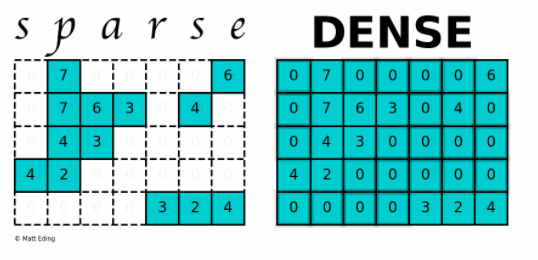
\includegraphics[width=\paperwidth,height=\paperheight,keepaspectratio]{../../pictures/sparse_dense.png}}
\url{https://matteding.github.io/2019/04/25/sparse-matrices/}
\end{frame}
}


\begin{frame}[standout]
Tomorrow we discuss how we can tokenize with a list comprehension (and that's often a good idea!). But what if we want to \emph{directly} get a DTM instead of lists of tokens?
\end{frame}


\begin{frame}[fragile]{OK, good enough, perfect?}
\begin{block}{scikit-learn's CountVectorizer (default settings)}
\begin{itemize}
	\item applies lowercasing
	\item deals with punctuation etc. itself
	\item minimum word length $>1$
	\item more technically, tokenizes using this regular expression: \texttt{r"(?u)\textbackslash b\textbackslash w\textbackslash w+\textbackslash b"} \footnote{?u = support unicode, \textbackslash b = word boundary}
\end{itemize}
\end{block}
\begin{lstlisting}
from sklearn.feature_extraction.text import CountVectorizer
cv = CountVectorizer()
dtm_sparse = cv.fit_transform(docs)
\end{lstlisting}
\end{frame}


\begin{frame}{OK, good enough, perfect?}
\begin{block}{CountVectorizer supports more}
\begin{itemize}
\item stopword removal
\item custom regular expression
\item or even using an external tokenizer
\item ngrams instead of unigrams
\end{itemize}
\end{block}
\tiny{see \url{https://scikit-learn.org/stable/modules/generated/sklearn.feature\_extraction.text.CountVectorizer.html}}

\pause
\begin{alertblock}{Best of both worlds}
\textbf{Use the Count vectorizer with a NLTK-based external tokenizer! (see book)}
\end{alertblock}
\end{frame}


\subsection{Pruning}

\begin{frame}{General idea}
\begin{itemize}
	\item Idea behind both stopword removal and tf$\cdot$idf: too frequent words are uninformative
	\item<2-> (possible) downside stopword removal: a priori list, does not take empirical frequencies in dataset into account
	\item<3-> (possible) downside tf$\cdot$idf: does not reduce number of features
\end{itemize}

\onslide<4->{Pruning: remove all features (tokens) that occur in less than X or more than X of the documents}
\end{frame}

\begin{frame}[fragile, plain]
CountVectorizer, only stopword removal
\begin{lstlisting}
from sklearn.feature_extraction.text import CountVectorizer, TfidfVectorizer
myvectorizer = CountVectorizer(stop_words=mystopwords)
\end{lstlisting}

CountVectorizer, better tokenization, stopword removal (pay attention that stopword list uses same tokenization!):
\begin{lstlisting}
myvectorizer = CountVectorizer(tokenizer = TreebankWordTokenizer().tokenize, stop_words=mystopwords)
\end{lstlisting}

Additionally remove words that occur in more than 75\% or less than $n=2$ documents:
\begin{lstlisting}
myvectorizer = CountVectorizer(tokenizer = TreebankWordTokenizer().tokenize, stop_words=mystopwords, max_df=.75, min_df=2)
\end{lstlisting}

All togehter: tf$\cdot$idf, explicit stopword removal, pruning
\begin{lstlisting}
myvectorizer = TfidfVectorizer(tokenizer = TreebankWordTokenizer().tokenize, stop_words=mystopwords, max_df=.75, min_df=2)
\end{lstlisting}


\end{frame}


\question{What is ``best''? Which (combination of) techniques to use, and how to decide?}




\end{document}


